%%%%%%%%%%%%%%%%%%%%%%%%%%%%%%%%%% Section 4: Proposed Approach %%%%%%%%%%%%%%%%%%%%%%%%%%%%%%%%%
\section{Proposed Approach}
\label{sec:Approach}
%Traditionally we can obtain the reference path $\mathcal{P}$ using the RRT sampling-based path-planning algorithm, depicted in Alg. \ref{alg:traditional_rrt}. As demonstrated, the algorithm receives as input the initial position of the agent, denoted as \( y(0) \), at time \( t = 0 \), along with the goal region \( \mathcal{G}_o \in \mathbb{R}^2 \) (e.g., the centroid of the target region \( \mathcal{G} \)) and the set of fire fronts \( \mathcal{O} \). The algorithm proceeds by incrementally constructing a tree \( V \), originating from the agent's initial state and expanding toward the goal region \( \mathcal{G}_o \). During each iteration, a point \( \nu_{\text{rand}} \) is randomly sampled from the space, and the tree is extended from its closest existing vertex \( \nu_{\text{nearest}} \) toward \( \nu_{\text{rand}} \), resulting in a new vertex \( \nu_{\text{new}} \), provided that the path does not intersect any fire fronts, ensuring navigational safety. The extension follows a predefined step size $\delta$, systematically guiding the tree's exploration of the space. This iterative process continues until either the tree successfully reaches the goal region (i.e., \( ||\nu_{\text{new}} - G_o||_2 \leq \epsilon \), where \( \epsilon > 0 \)) in which case the path is retrieved via backtracking, or the predefined iteration limit  $N$  is reached, resulting in the algorithm failing to converge.
%
%The RRT algorithm, while widely effective across various motion planning tasks, encounters several inherent challenges that can impact its performance. One significant limitation is low sampling efficiency, as traditional RRT often produces a high proportion of invalid or redundant samples. This inefficiency increases computational overhead and hampers the algorithm's ability to explore the search space effectively. Additionally, the resulting paths may include unnecessary detours or redundant nodes, which can lead to suboptimal path quality and increased traversal cost. 
%
%To address these limitations VLM-RRT utilizes LLMs as general purpose pattern matching machines, and integrates their reasoning capabilities into RRT search to guide the sampling process towards regions most likely to contain the optimal solution. 


Traditionally, we can obtain the reference path \( \mathcal{P} \) using the RRT sampling-based path-planning algorithm, depicted in Alg.~\ref{alg:traditional_rrt}. As demonstrated, the algorithm receives as input the initial position of the agent, denoted as \( y(0) \), at time \( t = 0 \), along with the goal region \( \mathcal{G}_o \in \mathbb{R}^2 \) (e.g., the centroid of the target region \( \mathcal{G} \)) and the set of fire fronts \( \mathcal{O} \). The algorithm proceeds by incrementally constructing a tree \( V \), originating from the agent's initial state and expanding toward the goal region \( \mathcal{G}_o \). During each iteration, a point \( \nu_{\text{rand}} \) is randomly sampled from the space, and the tree is extended from its closest existing vertex \( \nu_{\text{nearest}} \) toward \( \nu_{\text{rand}} \), resulting in a new vertex \( \nu_{\text{new}} \), provided that the path does not intersect any fire fronts, ensuring navigational safety. The extension follows a predefined step size \( \delta \), systematically guiding the tree's exploration of the space. This iterative process continues until either the tree successfully reaches the goal region (i.e., \( \|\nu_{\text{new}} - \mathcal{G}_o\|_2 \leq \epsilon \), where \( \epsilon > 0 \)), in which case the path is retrieved via backtracking, or the predefined iteration limit \( N \) is reached, resulting in the algorithm failing to converge.

The RRT algorithm, while widely effective across various motion planning tasks, encounters several inherent challenges that can impact its performance. One significant limitation is low sampling efficiency, as traditional RRT often produces a high proportion of invalid or redundant samples. This inefficiency increases computational overhead and hampers the algorithm's ability to explore the search space effectively. Additionally, the resulting paths may include unnecessary detours or redundant nodes, which can lead to suboptimal path quality and increased traversal cost.

To address these limitations, VLM-RRT utilizes LLMs as general-purpose pattern-matching machines and integrates their reasoning capabilities into the RRT search to guide the sampling process toward regions most likely to contain the optimal solution.






%%%%%%%%%%%%%%%%%%%%%%%%%%%%%%%%%%%%%%%%%%%% VLM RRT %%%%%%%%%%%%%%%%%%%%%%%%%%%%%%%%%%%%%%%%%%%%
\begin{algorithm}
\caption{VLM-RRT Algorithm}
\label{alg:vlm_rrt}
\begin{algorithmic}[1]
\Require $y(0), ~\mathcal{G}o,~\mathcal{O}$, $\delta, \gamma$
\State $V \gets {y(0)}$, $E \gets \emptyset$, $r \gets \emptyset$, $i \gets 0$
\While{$i < N$}
\State $E_{\text{current}} \gets \text{GetEnvironmentState}()$
\State $\alpha \gets \mathcal{U}(0,1)$ 
\If{$\alpha \leq \gamma$}
\State	$\hat{\nu} \gets \text{PickLeafNode}(V,E_{\text{current}})$
\State $d \gets \text{GetVLMdirection}(\hat{\nu},E_{\text{current}})$
\State $\nu_{\text{rand}} \gets \text{SampleStateVLM}(\hat{\nu},d, r, \theta)$
\Else
\State $\nu_{\text{rand}} \gets \text{SampleState}()$
\EndIf
\State $\nu_{\text{nearest}} \gets \text{NearestNeighbor}(V, \nu_{\text{rand}})$
\State $\nu_{\text{new}} \gets \text{Steer}(\nu_{\text{nearest}}, \nu_{\text{rand}}, \delta)$
\State $i \gets i + 1$
\If{$\text{PathFree}(\nu_{\text{new}},\nu_{\text{nearest}}, \mathcal{O})$}
\State $V \gets V \cup {\nu_{\text{new}}}$, $E \gets E \cup {(\nu_{\text{nearest}}, \nu_{\text{new}})}$
\EndIf
\If{$||\nu_{\text{new}} -  \mathcal{G}_o||_2 \leq \epsilon$}
\State $\mathcal{P} \gets \text{RetrievePlan}(V, E, \nu_{\text{new}})$
\State \Return $\mathcal{P}$
\EndIf
\EndWhile
\end{algorithmic}
\end{algorithm}
%%%%%%%%%%%%%%%%%%%%%%%%%%%%%%%%%%%%%%%%%%%% VLM RRT %%%%%%%%%%%%%%%%%%%%%%%%%%%%%%%%%%%%%%%%%%%%

%%%%%%%%%%%%%%%%%%%%%%%%%%%%%%%%%%%% System Achitecture %%%%%%%%%%%%%%%%%%%%%%%%%%%%%%%%%%%%%%%%%
\begin{figure*}
    \centering
    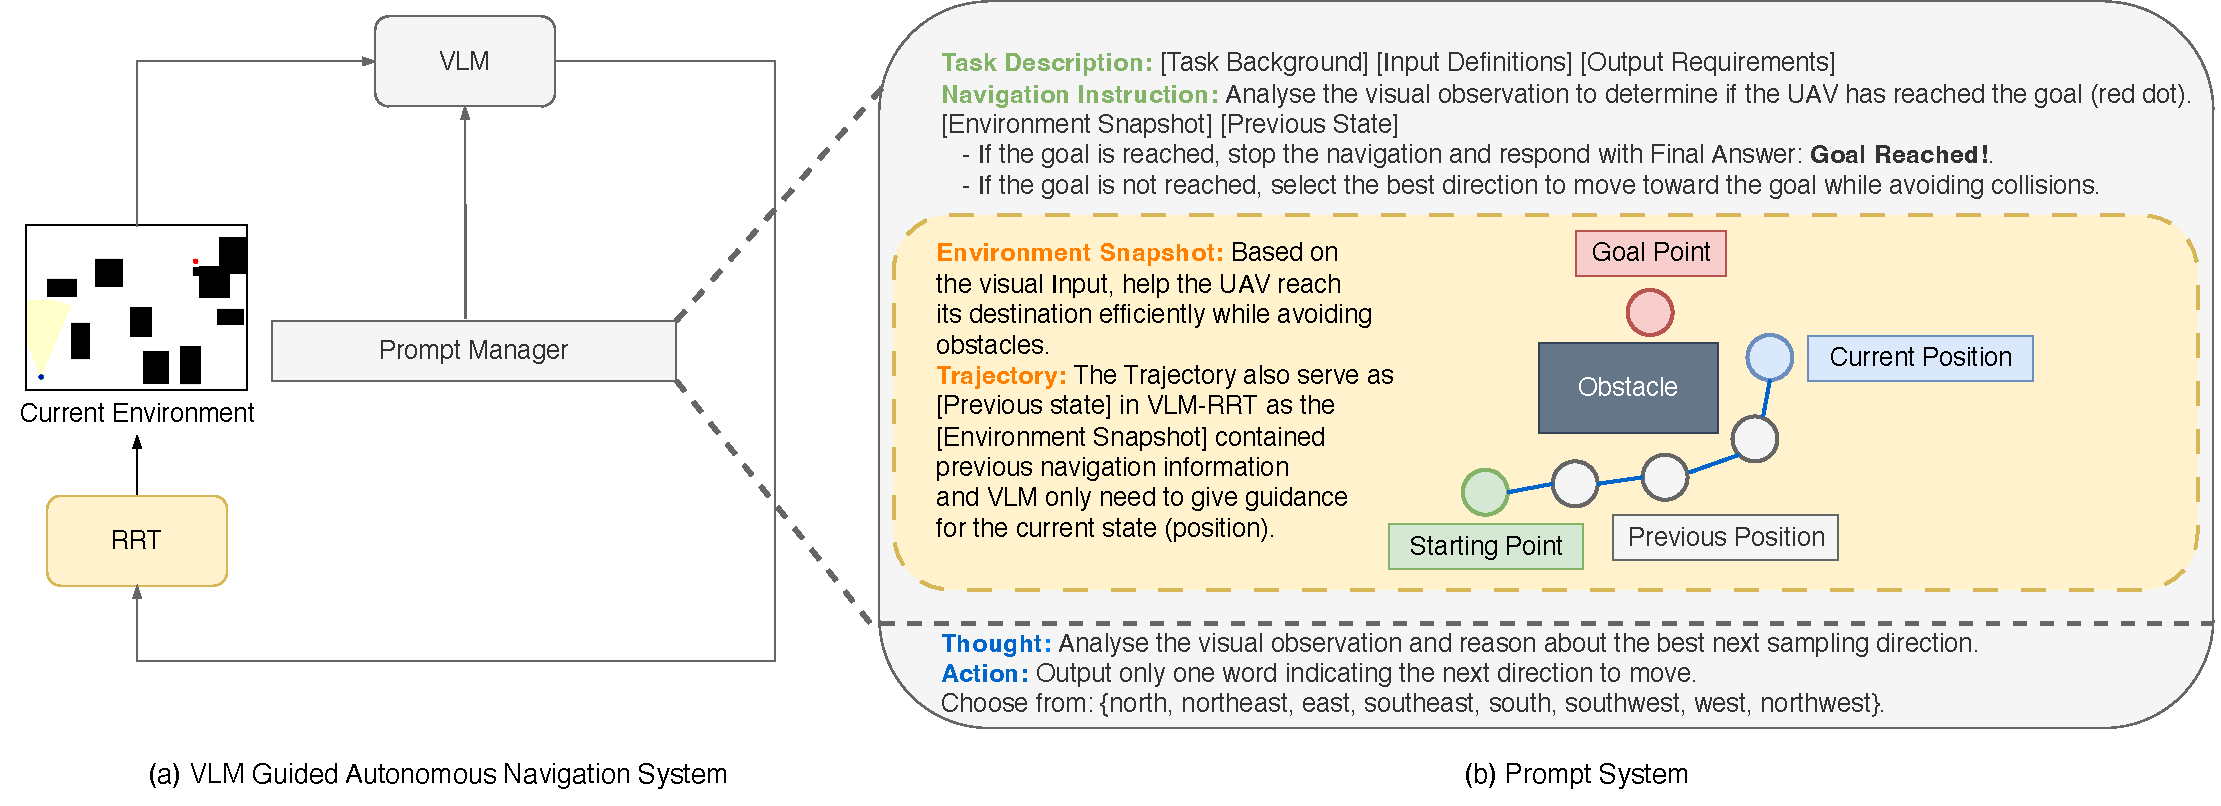
\includegraphics[width=1.0\textwidth]{images/system_achitecture2.pdf}
    \caption{Our basic system consists of two types of prompts, task descriptions and basic inputs. We match a snapshot of the current environment with the task instructions, incorporating the current navigation state and history into the prompt to activate the agent's global dynamic exploration capability.}
    \label{fig:system_achitecture}
\end{figure*}
%%%%%%%%%%%%%%%%%%%%%%%%%%%%%%%%%%%% System Achitecture %%%%%%%%%%%%%%%%%%%%%%%%%%%%%%%%%%%%%%%%%

\subsection{VLM-RRT}
\label{ssec:vlm_rrt}

The VLM-RRT algorithm, shown in Alg.~2, integrates VLMs into the sampling process of RRT. In this framework, VLMs serve as general-purpose pattern-matching and reasoning machines that extract contextual information from the current environment, as illustrated in Fig.~\ref{fig:system_achitecture}. The VLM output aims to improve sampling efficiency and steer the tree exploration toward regions that are more likely to yield an optimal path. In our context, ``optimal'' refers to the collision-free route that minimizes the total travel distance from the starting position to the goal region, ensuring the most efficient navigation.

At the start of each planning iteration, the algorithm captures the current state of the environment as an image \( E_{\text{current}} \) using the function \texttt{GetEnvironmentState}. This image encodes the locations of fire fronts \( \mathcal{O} \), the goal region, and the state of exploration represented by the tree \( V \). In this representation, the goal region and the leaf nodes in \( V \) are distinguished using different colors.

Subsequently, with probability \( \gamma \), the algorithm decides whether to take a VLM-informed exploration step. In Line 4, the random variable \( \alpha \) is drawn from the uniform distribution in the range \( (0,1) \). With probability \( \gamma \), the proposed approach randomly selects a leaf node \( \hat{\nu} \) from \( V \), as shown in Line 6 of Alg.~2, and then employs the VLM to determine the direction \( d \) in which the agent should move to reach the goal region, given the selected node \( \hat{\nu} \). This is achieved through the function \texttt{GetVLMdirection}, as shown in Line 7, which leverages the VLM via prompt engineering to detect the goal region and reason about the direction \( d \) the agent should take by analyzing the environment image \( E_{\text{current}} \).

The algorithm then proceeds by randomly sampling a new point \( \nu_{\text{rand}} \) from a sector \( \mathcal{R} \), centered at \( \hat{\nu} \), with direction \( d \), radius \( r \), and angle \( \theta \), as described in Line 8. Otherwise, with probability \( 1 - \gamma \), the algorithm follows the standard RRT sampling strategy, selecting \( \nu_{\text{rand}} \) from anywhere in the environment using the function \texttt{SampleState}, as shown in Line 10. Subsequently, the algorithm operates similarly to the original RRT, where the tree is expanded from its nearest existing vertex, \( \nu_{\text{nearest}} \), in the direction of \( \nu_{\text{rand}} \), generating a new vertex \( \nu_{\text{new}} \). This expansion occurs only if the resulting path does not intersect any fire fronts, thereby ensuring safe navigation toward the goal region. This iterative process continues until either the tree successfully reaches the goal region or the algorithm reaches the predefined iteration limit.




%%%%%%%%%%%%%%%%%%%%%%%%%%%%%%%%%%%% Prompt Engineering %%%%%%%%%%%%%%%%%%%%%%%%%%%%%%%%%%%%%%%%
\begin{figure*}
    \centering
    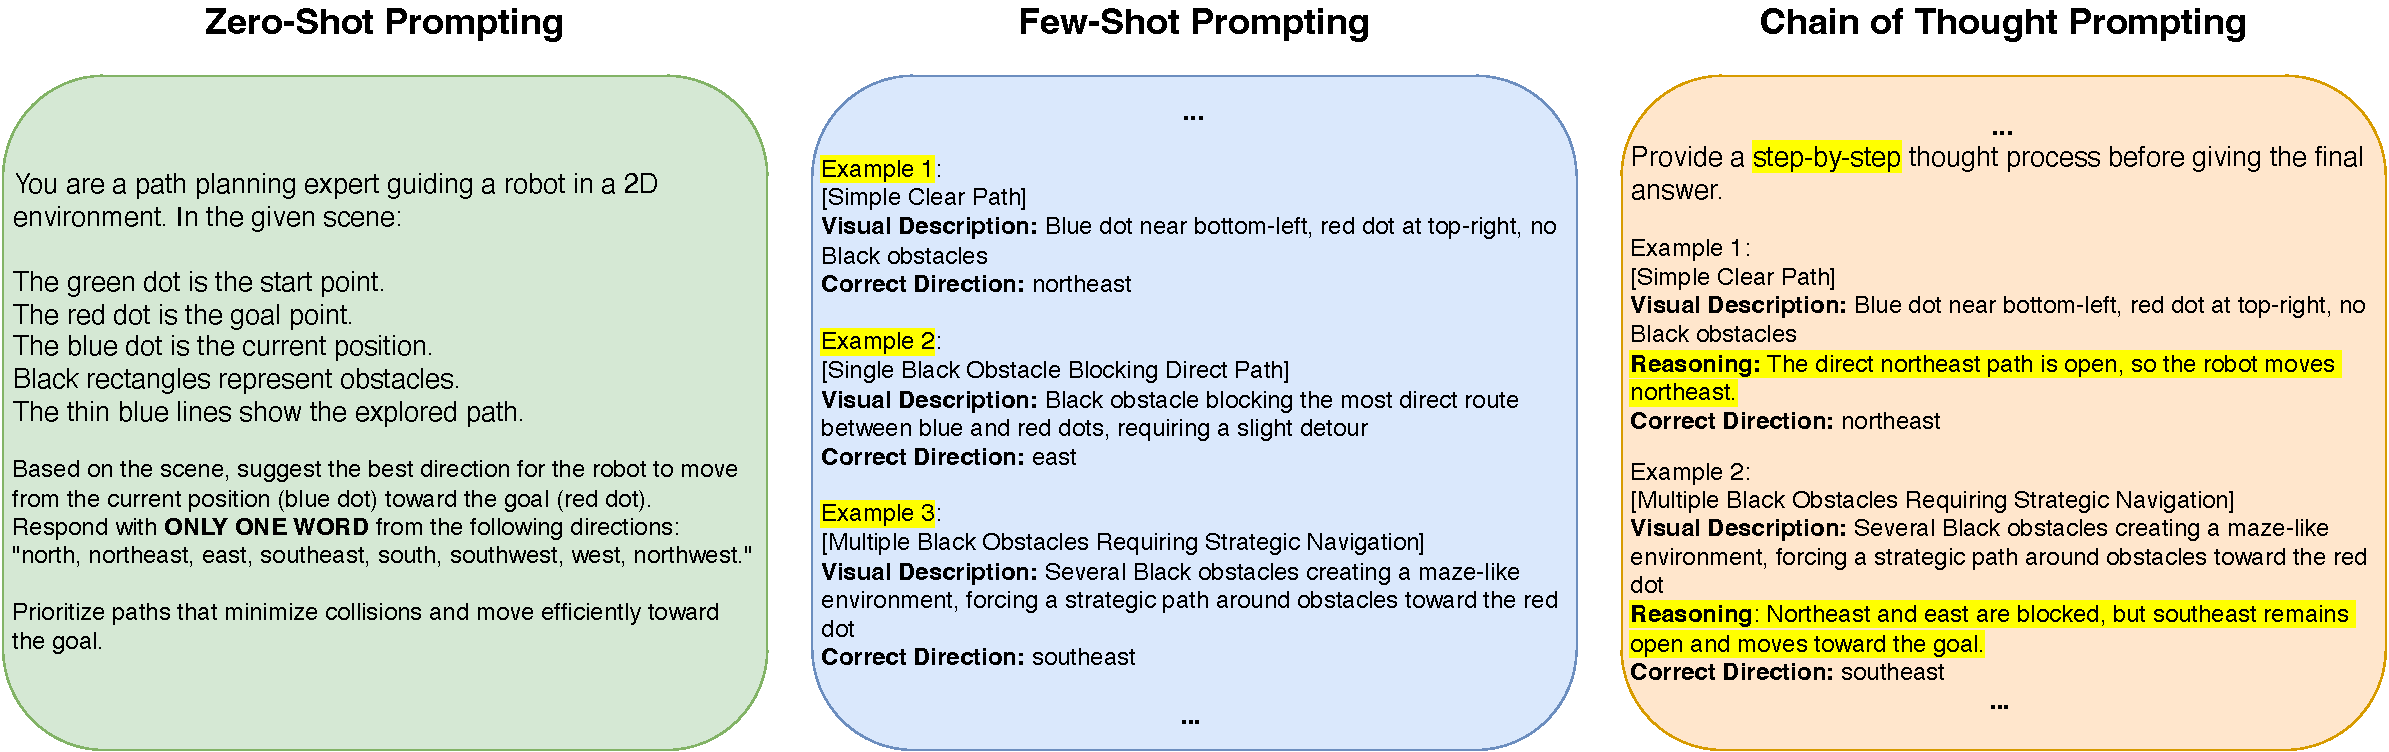
\includegraphics[width=1.0\textwidth]{images/Prompting.pdf}
    \caption{Comparison of different prompt engineering techniques for navigation decision-making.}
    \label{fig:prompt}
\end{figure*}
%%%%%%%%%%%%%%%%%%%%%%%%%%%%%%%%%%%% Prompt Engineering %%%%%%%%%%%%%%%%%%%%%%%%%%%%%%%%%%%%%%%%

\subsection{Prompt Engineering}

The prompt engineering methodology leverages the VLM's pattern-matching capabilities. As shown in Fig.~\ref{fig:system_achitecture}, our system implements structured prompts that combine task descriptions with environmental snapshots, incorporating both current navigation states and historical data. The prompt structure defines specific input parameters, output constraints, and environmental context for navigation guidance.

As demonstrated in Fig.~\ref{fig:prompt}, we experimented with three prompting techniques. Zero-shot prompting enables direct decision-making using only task instructions and current state information. Few-shot prompting augments this by including predefined example scenarios, ranging from unobstructed paths to multi-obstacle configurations, which serve as reference cases for similar navigation contexts. We integrated Chain of Thought (CoT) prompting~\cite{wei2022chain} to enhance the system's reasoning capabilities. The CoT framework structures the decision-making process into explicit steps: obstacle identification, relative position analysis, and path feasibility evaluation. This structured approach enables the model to systematically process environmental constraints before determining movement directions.









